\documentclass[12pt,a4paper]{article}
\usepackage[utf8]{inputenc}
\usepackage[american]{babel}
\usepackage{amsmath}
\usepackage{amsfonts}
\usepackage{amssymb}
\usepackage{mathtools}
\DeclarePairedDelimiter{\abs}{\lvert}{\rvert}
\newcommand{\pdiff}[2]{\frac{\partial #1}{\partial #2}}
\newcommand{\pdiffn}[3]{\frac{\partial^{#3} #1}{\partial #2^{#3}}}
\usepackage{geometry}
\usepackage[square]{natbib}
\usepackage[bookmarks,hidelinks]{hyperref}
\usepackage{subfiles}
\usepackage[numbib,nottoc]{tocbibind}
\usepackage{url}
\usepackage{todonotes}
\usepackage{siunitx}
\usepackage{tikz}
\usetikzlibrary{patterns}
\renewcommand{\epsilon}{\varepsilon}
\usepackage{titling}
\newcommand{\subtitle}[1]{
  \posttitle{
    \par\end{center}
    \begin{center}\large#1\end{center}
    \vskip0.5em}
}
\author{Marc John Bordier Dam}
\title{Using Numerical Methods to Explore Quantum Mechanics}
\linespread{1.3}

\begin{document}
\selectlanguage{american}
\maketitle

\section{Summary}
\todo[inline]{WRITE ME!}

\section{Introduction}
\todo[inline]{WRITE ME!}

\section{Schrödinger's Equation and its Solutions}
The most fundamental equation in quantum mechanics is the Schrödinger equation. It governs which functions are worthy of study, that is, which functions are allowed wave functions in a given potential. The time-dependent Schrödinger equation in one dimension is
\begin{equation}
i \hbar \pdiff{\Psi}{t} = - \frac{\hbar^2}{2 m} \pdiffn{\Psi}{x}{2} + V \Psi.
\end{equation}
To make solving the time-dependent Schrödinger equation easier we use separation of variables to obtain the time-independent Schrödinger equation
\begin{equation}
- \frac{\hbar^2}{2 m} \pdiffn{\psi}{x}{2} + V \psi = E \psi,
\end{equation}
where $\Psi = \psi e^{-\frac{i E t}{\hbar}}$.

The wave functions which are solutions to the time-independent Schrödinger euqation represent stationary states. These stationary states have the nice property that any function in Hilbert space can be written as a linear combination of them. Thus it is in many cases sufficient to work with the stationary states and linear combinations of them. Below we will present the stationary states along with their allowed energies for the infinite and finite square well.

\subsection{The Infinite Square Well}
\begin{figure}
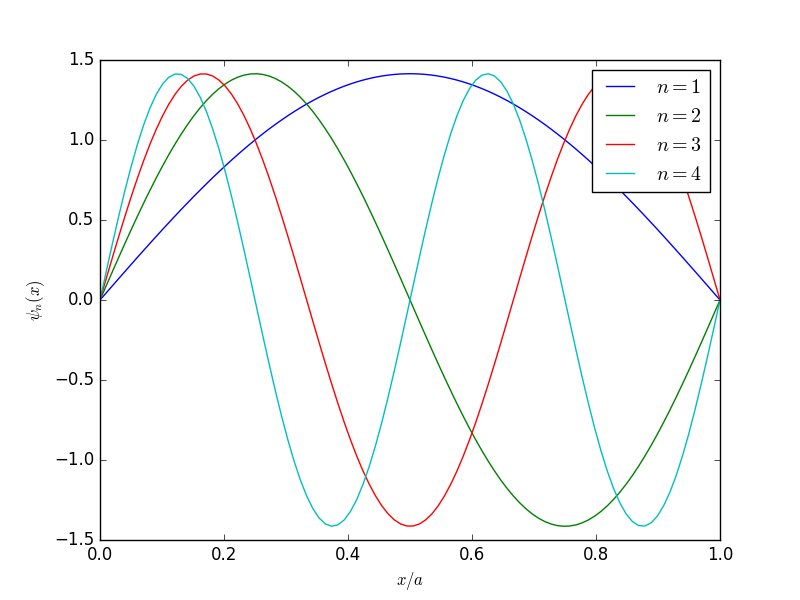
\includegraphics[width=\textwidth]{../Python/ISW_stationarySolutions.png}
\caption{Wave Functions in the Infinite Square well}
\label{fig:infiniteSquareWell}
\end{figure}

In the infinite square well the potential is given by
\begin{equation}
V = \begin{cases} 0, & 0 \leq x \leq a \\
                  \infty, & \text{otherwise} \end{cases}.
\end{equation}

Outside the well the wave function is $0$ and inside the well it is given by
\begin{equation}
\psi_n(x) = \sqrt{\frac{2}{a}} \sin \left( \frac{n \pi}{a} x \right),
\end{equation}
where $n$ is any positive integer. In the infinite square well the energy spectrum is discrete with the $n$th stationary state having the energy
\begin{equation}
E_n = \frac{n^2 \pi^2 \hbar^2}{2 m a^2}.
\end{equation}
Some of the wave functions are shown in figure~\ref{fig:infiniteSquareWell}.

\subsection{The Finite Square Well}
\begin{figure}
\missingfigure{Make a nice finite square well here}
\caption{Wave Functions in the Finite Square well}
\label{fig:finiteSquareWell}
\end{figure}

In the finite square well the potential is given by
\begin{equation}
V = \begin{cases} -V_0, & -a \leq x \leq a \\
                  0, & \text{otherwise} \end{cases},
\end{equation}
where $V_0$ is a positive number.

In the finite square well the wave function can be found both inside and outside the well. We also have both bound ($E < 0$) and scattering states ($E > 0$) in the finite square well.

The bound states come in two flavors: Even and odd. The even wave functions are given by
\begin{equation}
\psi_{even} (x) = \begin{cases} A e^{- \kappa x}, & a < x \\
                                A \frac{e^{- \kappa a}}{\cos la} \cos l x, & -a \leq x \leq a \\
                                A e^{\kappa x}, & x < -a \end{cases},
\end{equation}
where $A$ is a normalization constant, $\kappa = \frac{\sqrt{-2 m E}}{\hbar}$ and $l = \frac{\sqrt{2 m (E + V_0)}}{\hbar}$.

Similarly the odd wave functions are given by
\begin{equation}
\psi_{odd} (x) = \begin{cases} A e^{- \kappa x}, & a < x \\
                                A \frac{e^{- \kappa a}}{\sin la} \sin l x, & -a \leq x \leq a \\
                                - A e^{\kappa x}, & x < -a \end{cases},
\end{equation}
where again $A$ is a normalization constant, $\kappa = \frac{\sqrt{-2 m E}}{\hbar}$ and $l = \frac{\sqrt{2 m (E + V_0)}}{\hbar}$.

The energy spectrum of the bound states is discrete but can not be determined analytically. Defining $z = l a$ and $z_0 = \frac{a}{\hbar} \sqrt{2 m V_0}$ the allowed energies for the even wave functions can be found by solving the equation
\begin{equation}
\tan z = \sqrt{\left(\frac{z_0}{z} \right)^2 - 1}. \label{eq:evenEnergy}
\end{equation}
Likewise the allowed energies for the odd wave functions can be found by solving the equation
\begin{equation}
- \cot z = \sqrt{\left(\frac{z_0}{z} \right)^2 - 1}. \label{eq:oddEnergy}
\end{equation}
Some of the wave functions for the bound states are shown in figure~\ref{fig:finiteSquareWell}.

The wave functions for the scattering states are given by
\begin{equation}
\psi(x) = \begin{cases} F e^{ikx} & a < x \\
                        C \sin lx + D \cos lx & -a \leq x \leq a \\
                        A e^{ikx} + B e^{-ikx} & x < -a \end{cases},
\end{equation}
where $A$ is a normalization constant and
\begin{align*}
k &= \frac{\sqrt{2 m E}}{\hbar}, \\
l &= \frac{\sqrt{2 m (E + V_0)}}{\hbar}, \\
B &= i \frac{\sin 2 la}{2 kl} \left( l^2 - k^2 \right) F, \\
C &= \left( \sin la + i \frac{k}{l} \cos la \right) e^{ika} F, \\
D &= \left( \cos la - i \frac{k}{l} \sin la \right) e^{ika} F, \\
F &= \frac{e^{-2ika}}{\cos 2la - i \frac{k^2 + l^2}{2kl} \sin 2la} A.
\end{align*}
For the scattering states we observe reflection and transmission through the well wall.

The energy spectrum of the scattering states is continuous and thus any positive energy is allowed.

\section{Quantum Mechanics in Reduced Units}
When doing simulations we want to work with the physical quantities in reduced units. We do this for two reasons: We don't have to keep track of the units on everything and quantities in reduced units tend to be of a reasonable order of magnitude.

In our simulations we have three constants: The particle mass $m_0$, the well width $a$ and Planck's constant $\hbar$. In our system of reduced units these will all be equal to $1$. With these three constants we can derive the reduced units for the remaining relevant quantities in our simulation. The relevant quantities are shown in table~\ref{tab:reducedUnits}, where the real values for an electron in a $\pi$-bond in an ethylene molecule is also shown.

\begin{table}
\caption{Reduced Units (subscript $r$ denotes the quantity in real units)}
\label{tab:reducedUnits}
\begin{tabular}{c|ccc}
Quantity (Q.) & Q. in R. U. & Characteristic Q. & Electron in $\pi$-bond \\ 
\hline 
Length, $x$ & $\frac{x_r}{a}$ & $a$ & $\SI{1,34}{\angstrom}$ \\ 
Mass, $m$ & $\frac{m_r}{m_0}$ & $m_0$ & $m_e = \SI{9,109e-31}{\kilo\gram}$ \\ 
Time, $t$ & $\frac{t_r}{t_0}$ & $t_0 = \frac{m_0 a^2}{\hbar}$ & $\SI{1,55e-16}{\second}$ \\ 
Energy, $E$ & $\frac{E_r}{E_0}$ & $E_0 = \frac{\hbar^2}{m_0 a^2}$ & $\SI{6,80e-19}{\joule}$ \\ 
Velocity, $v$ & $\frac{v_r}{v_0}$ & $v_0 = \frac{\hbar}{m_0 a}$ & $\SI{8,64e5}{\meter\per\second}$ \\ 
Momentum, $p$ & $\frac{p_r}{p_0}$ & $p_0 = \frac{\hbar}{a}$ & $\SI{7,87e-25}{\meter\kilogram\per\second}$ \\ 
\end{tabular} 
\end{table}

\subsection{Schrödinger's Equation in Reduced Units}
Since $m$ and $\hbar$ both are equal to $1$ in our system of reduced units the time-dependent Schrödinger equation takes the form
\begin{equation}
i \pdiff{\Psi}{t} = - \frac{1}{2} \pdiffn{\Psi}{x}{2} + V \Psi,
\end{equation}
where $t$, $x$ and $V$ are all in reduced units. Likewise the time-indepedent Schrödinger equation takes the form
\begin{equation}
- \frac{1}{2} \pdiffn{\psi}{x}{2} + V \psi = E \psi,
\end{equation}
where again $x$, $V$ and $E$ are all in reduced units and $\Psi = \psi e^{i E t}$. The stationary wave functions in the infinite square well along with the allowed energies take the form
\begin{equation}
\psi_n(x) = \sqrt{2} \sin (n \pi x), \quad E_n = \frac{n^2 \pi^2}{2}.
\end{equation}
The wave functions representing bound stationary states take the form
\begin{equation}
\psi_{even}(x) = \begin{cases} A e^{-\sqrt{-2 E} x}, & 1 < x \\
                               A \frac{e^{-\sqrt{-2 E}}}{\cos \sqrt{2(E + V_0)}} \cos \left( \sqrt{2(E + V_0)} x \right), & -1 \leq x \leq 1 \\
                               A e^{-\sqrt{-2 E} x}, & x < -1 \end{cases}
\end{equation}
and
\begin{equation}
\psi_{odd}(x) = \begin{cases} A e^{-\sqrt{-2 E} x}, & 1 < x \\
                              A \frac{e^{-\sqrt{-2 E}}}{\sin \sqrt{2(E + V_0)}} \sin \left( \sqrt{2(E + V_0)} x \right), & -1 \leq x \leq 1 \\
                              -A e^{-\sqrt{-2 E} x}, & x < -1 \end{cases}.
\end{equation}
These equations along with equation~\eqref{eq:evenEnergy} and equation~\eqref{eq:oddEnergy} in reduced units is what will form the basis of our numerical investigations of the infinite and finite square well.

An idealized model of the $\pi$-bond in an ethylene molecule is an infinite square well where the width of the well is the length of a bond. The particle confined in the well then corresponds to an electron confined in a $\pi$-bond. The bond length between the two carbon atoms in ethylene is about $\SI{1.34}{\angstrom}$ and the mass of the electron is about $m_e = \SI{9.109e-31}{\kilo\gram}$. Using these numbers we can make a conversion table (table~\ref{tab:reducedUnits}) which allows us to convert from reduced units in our simulation to the real world example of an electron in a $\pi$-bond in an ethylene molecule.

\section{Numerical Methods}
Python

Numpy

Matplotlib

Trapz

Gradient

Newton's method

Code structure

Fourier's trick (projections)

\section{Numerical Results and Discussions}

\section{Appendix}
ALL THE CODE!!!!
\end{document}
